\documentclass{article}

\usepackage{graphicx}
\usepackage{tikz}
\usepackage{tikzsymbols}
\usetikzlibrary{calc,patterns,shapes.geometric}
\pagestyle{empty}
\usepackage[margin=0pt]{geometry}
\geometry{papersize={14in,12in}}

\def\centerarc[#1](#2)(#3:#4:#5){\draw[#1] ($(#2)+({#5*cos(#3)},{#5*sin(#3)})$) arc (#3:#4:#5);}

\begin{document}
	\begin{figure}
		\centering
		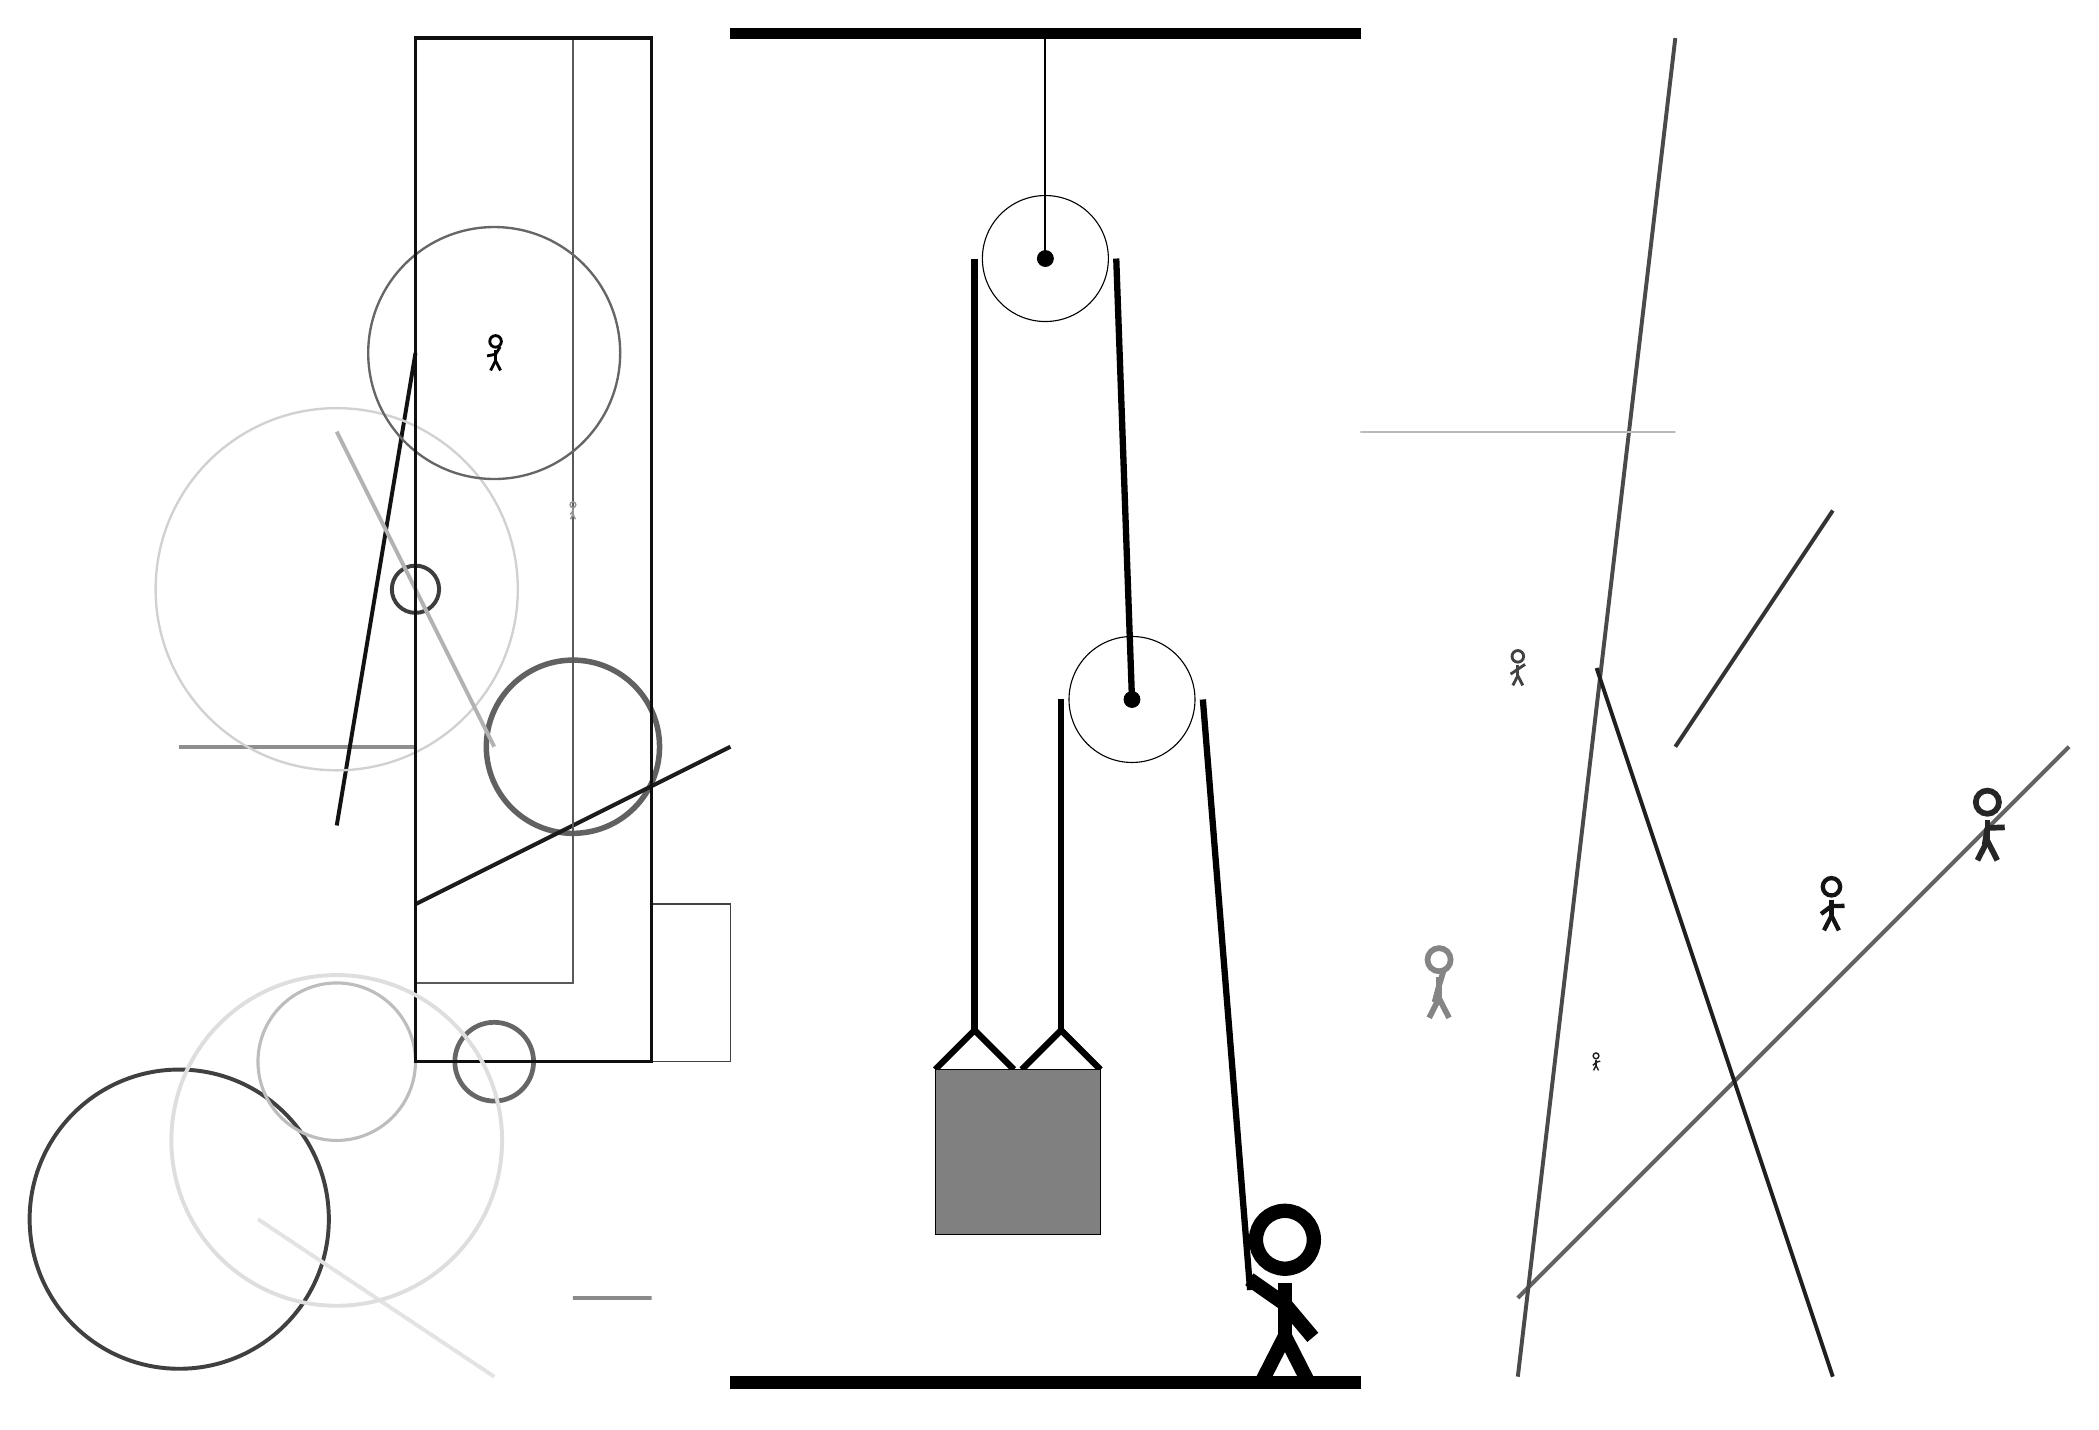
\begin{tikzpicture}
			%%%%% START %%%%%
			
			\draw[fill=black] (-2, 14) rectangle (6, 14.125);
			
			\draw[line width=0.5mm, color=black!44](-6, 5) -- (-9, 5);
			
			\draw [line width=0.7mm, color=black!62](-4, 5) circle (1.1);
			\draw[line width=0.5mm, color=black!61](8, -2) -- (15, 5);
			\draw[line width=0.5mm, color=black!89](-6, 3) -- (-2, 5);
			
			\node[line width=0.7mm, color=black!85] at (14, 4) {\Strichmaxerl[4][81][2]};
			
			\node[line width=0.6mm, color=black!74] at (8, 6) {\Strichmaxerl[2][34][34]};
			
			\draw[line width=0.5mm, color=black!93](-6, 10) -- (-7, 4);
			
			\draw [line width=0.3mm, color=black!18](-7, 7) circle (2.3);
			\draw [line width=0.5mm, color=black!76](-6, 7) circle (0.3);
			
			\draw[line width=0.3mm, color=black!65] (-4, 14) rectangle (-6, 2);
			\draw[line width=0.2mm, color=black!74] (-3, 1) rectangle (-2, 3);
			
			\node[line width=0.7mm, color=black!48] at (7, 2) {\Strichmaxerl[4][75][73]};
			\draw [line width=0.5mm, color=black!75](-9, -1) circle (1.9);
			
			\draw[line width=0.5mm, color=black!46] (-4, -2) rectangle (-3, -2);
			\draw[line width=0.5mm, color=black!30](-7, 9) -- (-5, 5);
			\draw[line width=0.5mm, color=black!71](10, 14) -- (8, -3);
			
			\draw[line width=0.5mm, color=black!11](-5, -3) -- (-8, -1);
			\draw[line width=0.3mm, color=black!27] (6, 9) rectangle (10, 9);
			\draw [line width=0.4mm, color=black!26](-7, 1) circle (1.0);
			
			\node[line width=0.5mm, color=black!88] at (9, 1) {\Strichmaxerl[1][44][16]};
			\node[line width=0.2mm, color=black!92] at (12, 3) {\Strichmaxerl[3][37][1]};
			
			\node[line width=0.3mm, color=black!42] at (-4, 8) {\Strichmaxerl[1][50][89]};
			\draw [line width=0.3mm, color=black!60](-5, 10) circle (1.6);
			\node[line width=0.7mm, color=black!99] at (-5, 10) {\Strichmaxerl[2][11][58]};
			\draw [line width=0.6mm, color=black!60](-5, 1) circle (0.5);
			\draw[line width=0.4mm, color=black!94] (-3, 14) rectangle (-6, 1);
			
			\draw[line width=0.5mm, color=black!80](10, 5) -- (12, 8);
			\draw [line width=0.5mm, color=black!13](-7, 0) circle (2.1);
			\draw[line width=0.5mm, color=black!88](9, 6) -- (12, -3);
			
			
			\draw (2, 11.2) circle (0.8);
			\draw[fill=black] (2, 11.2) circle (0.1);
			\draw[thick] (2, 11.2) -- (2, 14);
			
			\draw (3.1, 5.6) circle (0.8);
			\draw[fill=black] (3.1, 5.6) circle (0.1);
			
			\draw[line width = 0.8mm]  (0.6, 0.9) -- (1.1, 1.4) -- (1.6, 0.9);
			\draw[line width = 0.8mm]  (1.7, 0.9) -- (2.2, 1.4) -- (2.7, 0.9);
			\draw[fill=black!50] (0.6, 0.9) rectangle (2.7, -1.2);
			
			\draw[line width = 0.8mm] (1.1, 11.2) -- (1.1, 1.4);
			\centerarc[line width = 0.8mm](2, 11.2)(0:180:0.9);
			\draw[line width = 0.8mm] (2.9, 11.2) -- (3.1, 5.6);
			\draw[line width = 0.8mm] (2.2, 5.6) -- (2.2, 1.4);
			\centerarc[line width = 0.8mm](3.1, 5.6)(0:180:0.9);
			\draw[line width = 0.8mm] (4.0, 5.6) -- (4.6, -1.9);
			
			\node at (5, -2) {\Strichmaxerl[10][-35][-50]};
			
			\draw[fill=black] (-2, -3) rectangle (6, -3.15);
			
			%%%%% END %%%%%
		\end{tikzpicture}
	\end{figure}	
\end{document}